\documentclass{article}
\input{../../preamble.tex}

\usepackage{fancyhdr}
\usepackage{cancel}
\usepackage[margin=1in, headheight=50pt]{geometry}
\pagestyle{fancy}
\lhead{\textbf{Ph22 Set 1}}
\chead{}
\rhead{Aritra Biswas}
\setlength{\headsep}{20pt}

\begin{document}

\section{Convergence of the secant method}

\begin{prop}
    The order of convergence of the secant method is the golden ratio
    $\phi = (1 + \sqrt5)/2$.
\end{prop}

\begin{proof}
We are trying to find a root of a function $f(x)$. Let $\hat x$ be the
root we seek, such that $f(\hat x) = 0$. The Newton-Rhaphson method produces
a series of guesses $x_i$ which iterate as:
\begin{align}
    x_{i+1} = x_i - {f(x_i) \over f'(x_i)}.
\end{align}
In the secant method, we approximate $f'(x_i)$ using the slope of a secant:
\begin{align}
    x_{i+1} = x_i - f(x_i) {x_i - x_{i-1} \over f(x_i) - f(x_{i-1})}.
\end{align}
Let $\ep_i \equiv x_i - \hat x$. After our guesses $x_i$ are close, we can
approximate $f(x_i)$ with a Taylor expansion in the error:
\begin{align}
    f(x_i) = f(\hat x + \ep_i)
    \approx \cancel{f(\hat x)} + \ep_i f'(\hat x)
    + \ep_i^2 {f''(\hat x) \over 2}.
\end{align}
We can express (2) in terms of the errors and use this approximation to
obtain a recursion relation for the errors $\ep_i$:
\begin{align}
    \ep_{i+1} &= \ep_i - f(x_i) {\ep_i - \ep_{i-1} \over f(x_i) - f(x_{i-1})}.
\end{align}
We'll anticipate
the geometric nature of the recurrence relation by isolating the ratio
$\ep_{i + 1} / \ep_i$.
For simplicity, let's abstract away the constants
$A \equiv f'(\hat x)$, $B \equiv f''(\hat x) / 2$, and $C \equiv B/A$:
\begin{align}
    {\ep_{i+1} \over \ep_i} &=
    1 - (A + B\ep_i)
    {
        \ep_i - \ep_{i-1}
        \over
        A(\ep_i - \ep_{i-1}) + B(\ep_i^2 - \ep_{i-1}^2)
    }.
\end{align}
Factoring $\ep_i - \ep_{i-1}$ out of the fraction yields:
\begin{align}
    {\ep_{i+1} \over \ep_i} &=
    1 - (A + B\ep_i)
    {
        1
        \over
        A + B(\ep_i + \ep_{i-1})
    }
    = 1 - (1 + C\ep_i)
    {
        1
        \over
        1 + C(\ep_i + \ep_{i-1})
    }.
\end{align}
Here we note that $\eta \equiv C(\ep_i + \ep_{i - 1}) \ll 1$ and
use $(1 + \eta)^{-1} \approx 1 - \eta$:
\begin{align}
    {\ep_{i+1} \over \ep_i} &=
    1 - (1 + C\ep_i)
    (1 - C\ep_i - C\ep_{i-1})
    = 1 - \bigg[1 - C\ep_i - C\ep_{i-1} + C\ep_i + O(\ep_i^2)\bigg]
    \approx C \ep_{i - 1}.
\end{align}
Thus we have our desired recurrence relation:
\begin{align}
    \ep_{i + 1} \approx C \ep_i \ep_{i - 1}.
\end{align}
Now we assume that $\ep_{i + 1} = D \ep_i^r$ for all $i$, which
allows us to replace:
\begin{align}
    \ep_{i + 1} = D \ep_i^r = D (D \ep_{i - 1}^r)^r =
    D^{r + 1} \ep_{i - 1}^{r^2}.
\end{align}
This yields:
\begin{align}
    D^{r + 1} \ep_{i - 1}^{r^2}
    = C (D \ep_{i-1}^r)\ep_{i - 1}
    = CD \ep_{i-1}^{r + 1}.
\end{align}
Since this equation must be true for all $i$, corresponding
powers and coefficients of $\ep_{i-1}$ must match and we get:
\begin{align}
    D^{r + 1} = CD,
    \sp{and} r^2 = r + 1.
\end{align}
The latter is the defining polynomial for the golden ratio:
$r = \phi$ is its positive solution. We exclude the negative solution
since $\ep_i \ll 1$, so $r < 0$ would have $\ep_{i+1} > \ep$ and
the method would not converge. $\square$
\end{proof}

\section{Testing convergence on root-finding methods}

We define a test function $f_c(x) = \sin x - c$,
with an analytical root of $\hat x = \arcsin c$. We will test the convergence
rates of our three root-finding algorithms (bisection, Newton-Rhaphson,
and secant) on this function with $c = 4 \times 10^{-3}$.

\begin{table}[ht!]\centering
    \begin{tabular}{l | r | r | r}
        \textbf{Method} & Initial Guesses & Result & Difference
        from Analytical\\\hline
        Analytical & & 0.00400001066674 & 0 \\
        Bisection & -0.5, 1.0& 0.00400000996888
        & $-6.97866629068 \times 10^{-10}$ \\
        Newton-Raphson & 1.0 & 0.00400001066674
        & $-8.67361737988 \times 10^{-19}$\\
        Secant & -0.5, 1.0 & 0.00400001066674 & 0.0
    \end{tabular}
    \label{results}
    \caption{Results for $f_c(x) = \sin x - c$
    with $c = 4 \times 10^{-3}$ and requested
    tolerance $10^{-8}.$}
\end{table}

\begin{figure}[ht!]\centering
    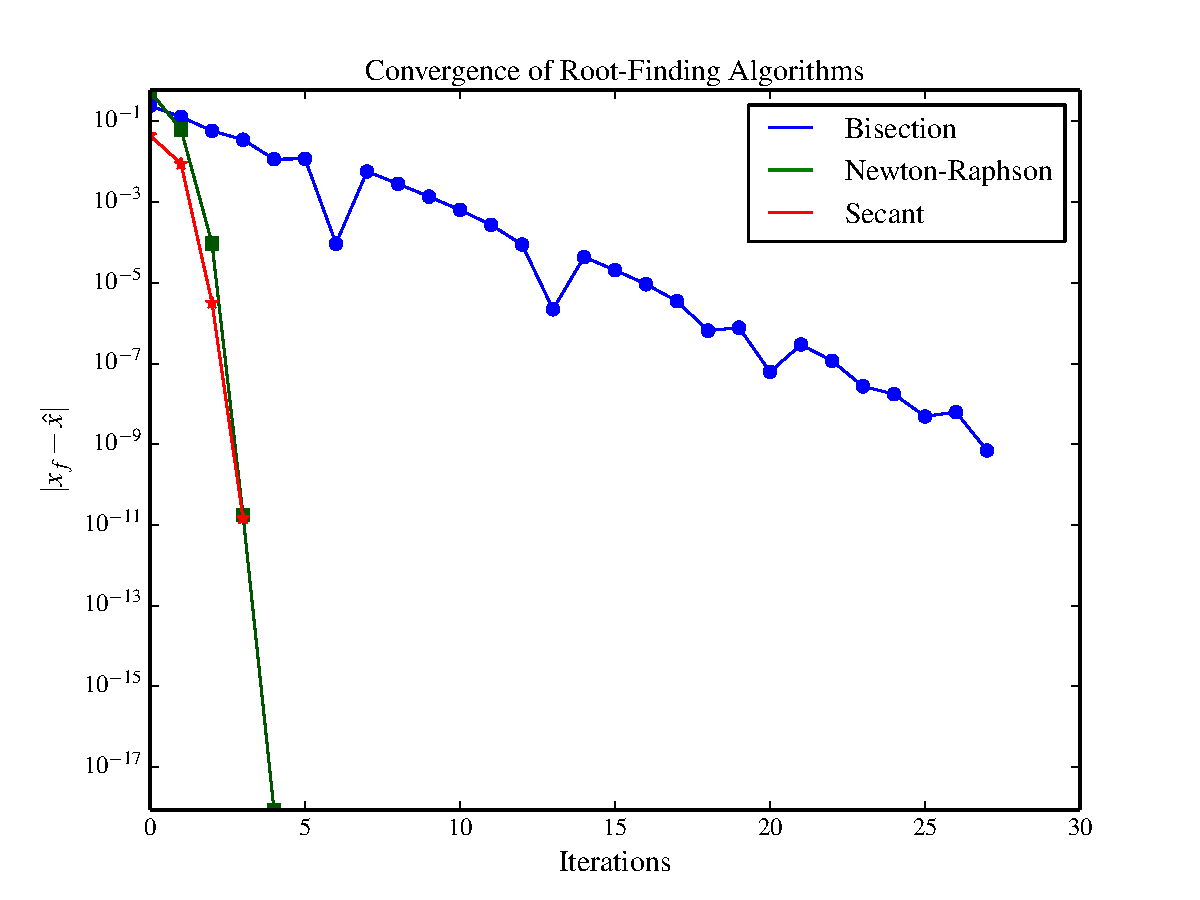
\includegraphics[width=0.8\textwidth]{convergence.pdf}
    \label{convergence}
    \caption{Absolute difference $|x_f - \hat x|$,
        where $x_f$ is the final result and $\hat x$ is the analytical root,
    as a function of number of iterations for all methods.}
\end{figure}

\section{Orbit of 1913+16 binary pulsar}

Elliptical orbits can be parametrized in terms of the eccentric anomaly,
or angle around the ellipse, $\xi$:
\begin{align}
    x(\xi) = a(\cos\xi - e),
    \sp{}
    y(\xi) = a \sqrt{1 - e^2} \sin\xi,
    \sp{}
    t(\xi) = {T \over 2\pi} (\xi - e \sin\xi),
\end{align}
where $a$ is the projected semimajor axis, $T$ the period, and $e$
the eccentricity.
Since $\xi$ varies from $0$ to $2\pi$, we need not include a time calculation
to calculate the shape of the orbit. However, to obtain $x(t)$ and $y(t)$
numerically, we use the secant method to invert the last equation and
numerically find $\xi(t)$, then inserting this parameter into $x(\xi)$
and $y(\xi)$. The resulting orbit is shown in Figure 2. A projection angle
of $\phi = 3\pi / 2$ resulted in the best visual agreement for the
radial velocity curve, shown in Figure 3.

\begin{figure}[ht!]\centering
    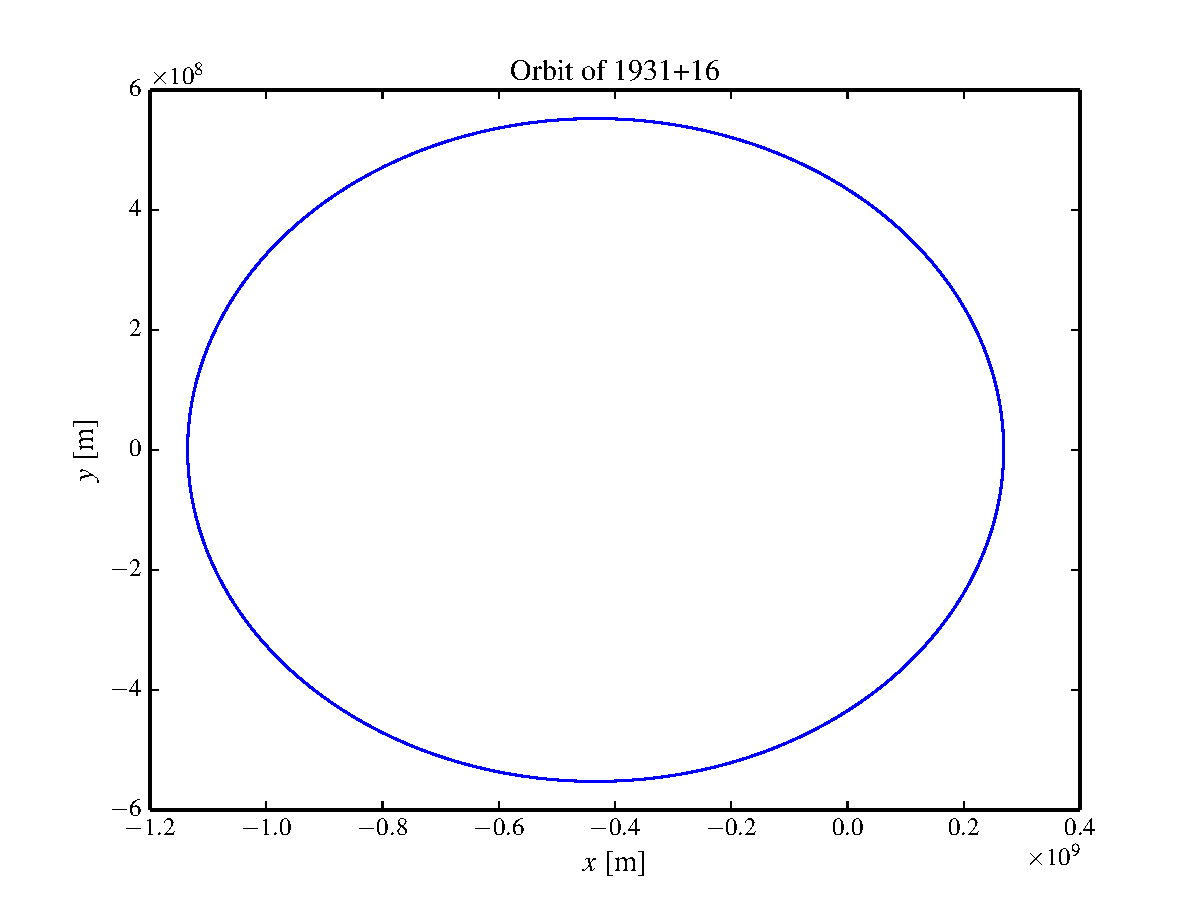
\includegraphics[width=0.8\textwidth]{orbit.pdf}
    \label{orbit}
    \caption{Orbit shape calculated through time.}
\end{figure}

\begin{figure}[ht!]\centering
    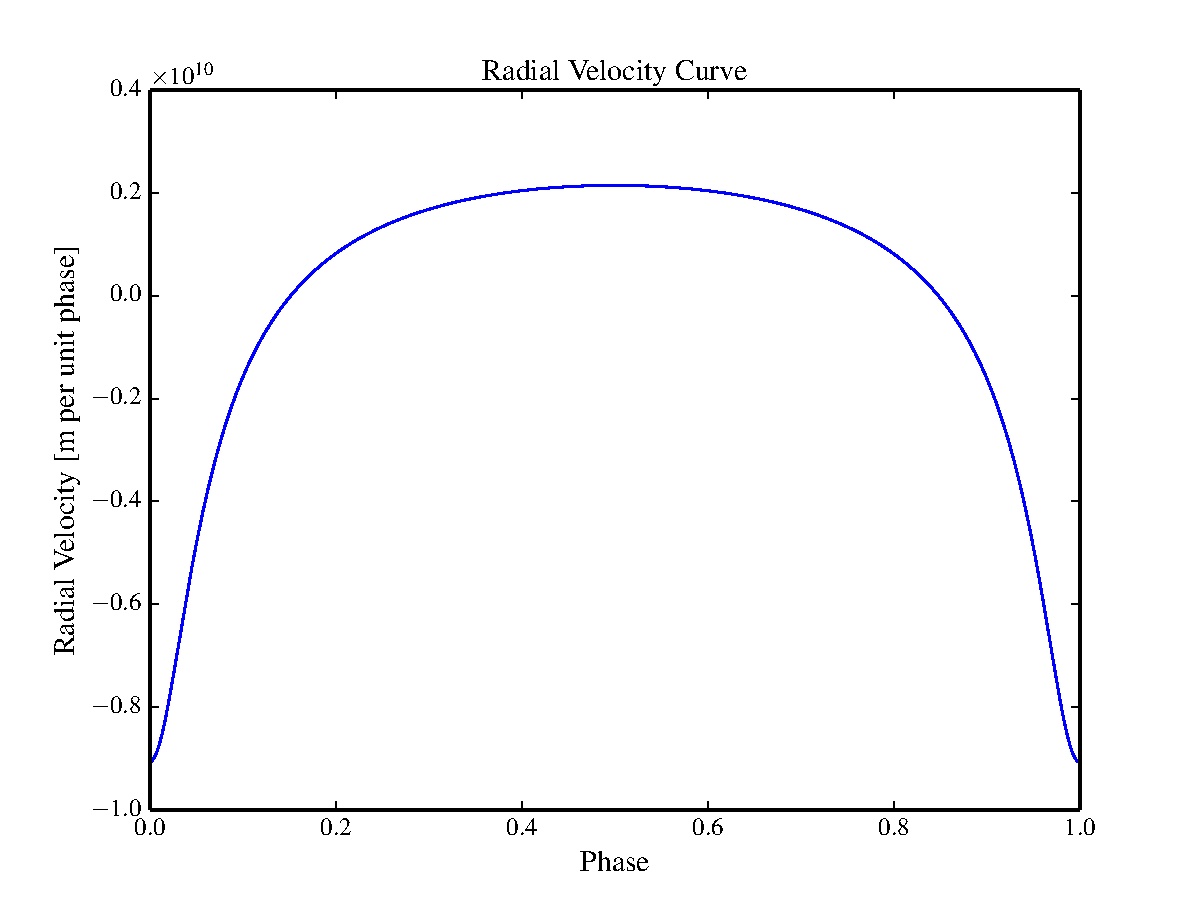
\includegraphics[width=0.8\textwidth]{vr_curve.pdf}
    \label{orbit}
    \caption{Radial velocity curve, projected at a viewing angle
    of $3\pi/2$.}
\end{figure}



\end{document}
